\chapter{Il software QSapecNG}

In questa appendice viene fatta una breve panoramica sull'ambiente per il disegno e l'analisi che accompagna il software di risoluzione, entrambi sviluppati durante il lavoro di tesi. Quella che segue non vuole essere una guida per l'utente all'uso di QSapecNG ma semplicemente un'introduzione a ciò che esso offre, aiutata dall'uso di alcune immagini del software in esecuzione.

Innanzitutto il \textit{design} è volto a rendere l'interfaccia maggiormente user-friendly, permettendo a QSapecNG di penetrare in ambienti dove i diversi soggetti non abbiano necessariamente uno stesso grado di esperienza nell'uso di strumenti del genere. Questo permette tanto al neofita quanto all'esperto di utilizzare QSapecNG ai propri scopi, con una curva di apprendimento legata alle conoscenze del singolo.

\paragraph{}

\begin{figure}[hb]
 \centering
 \subfloat{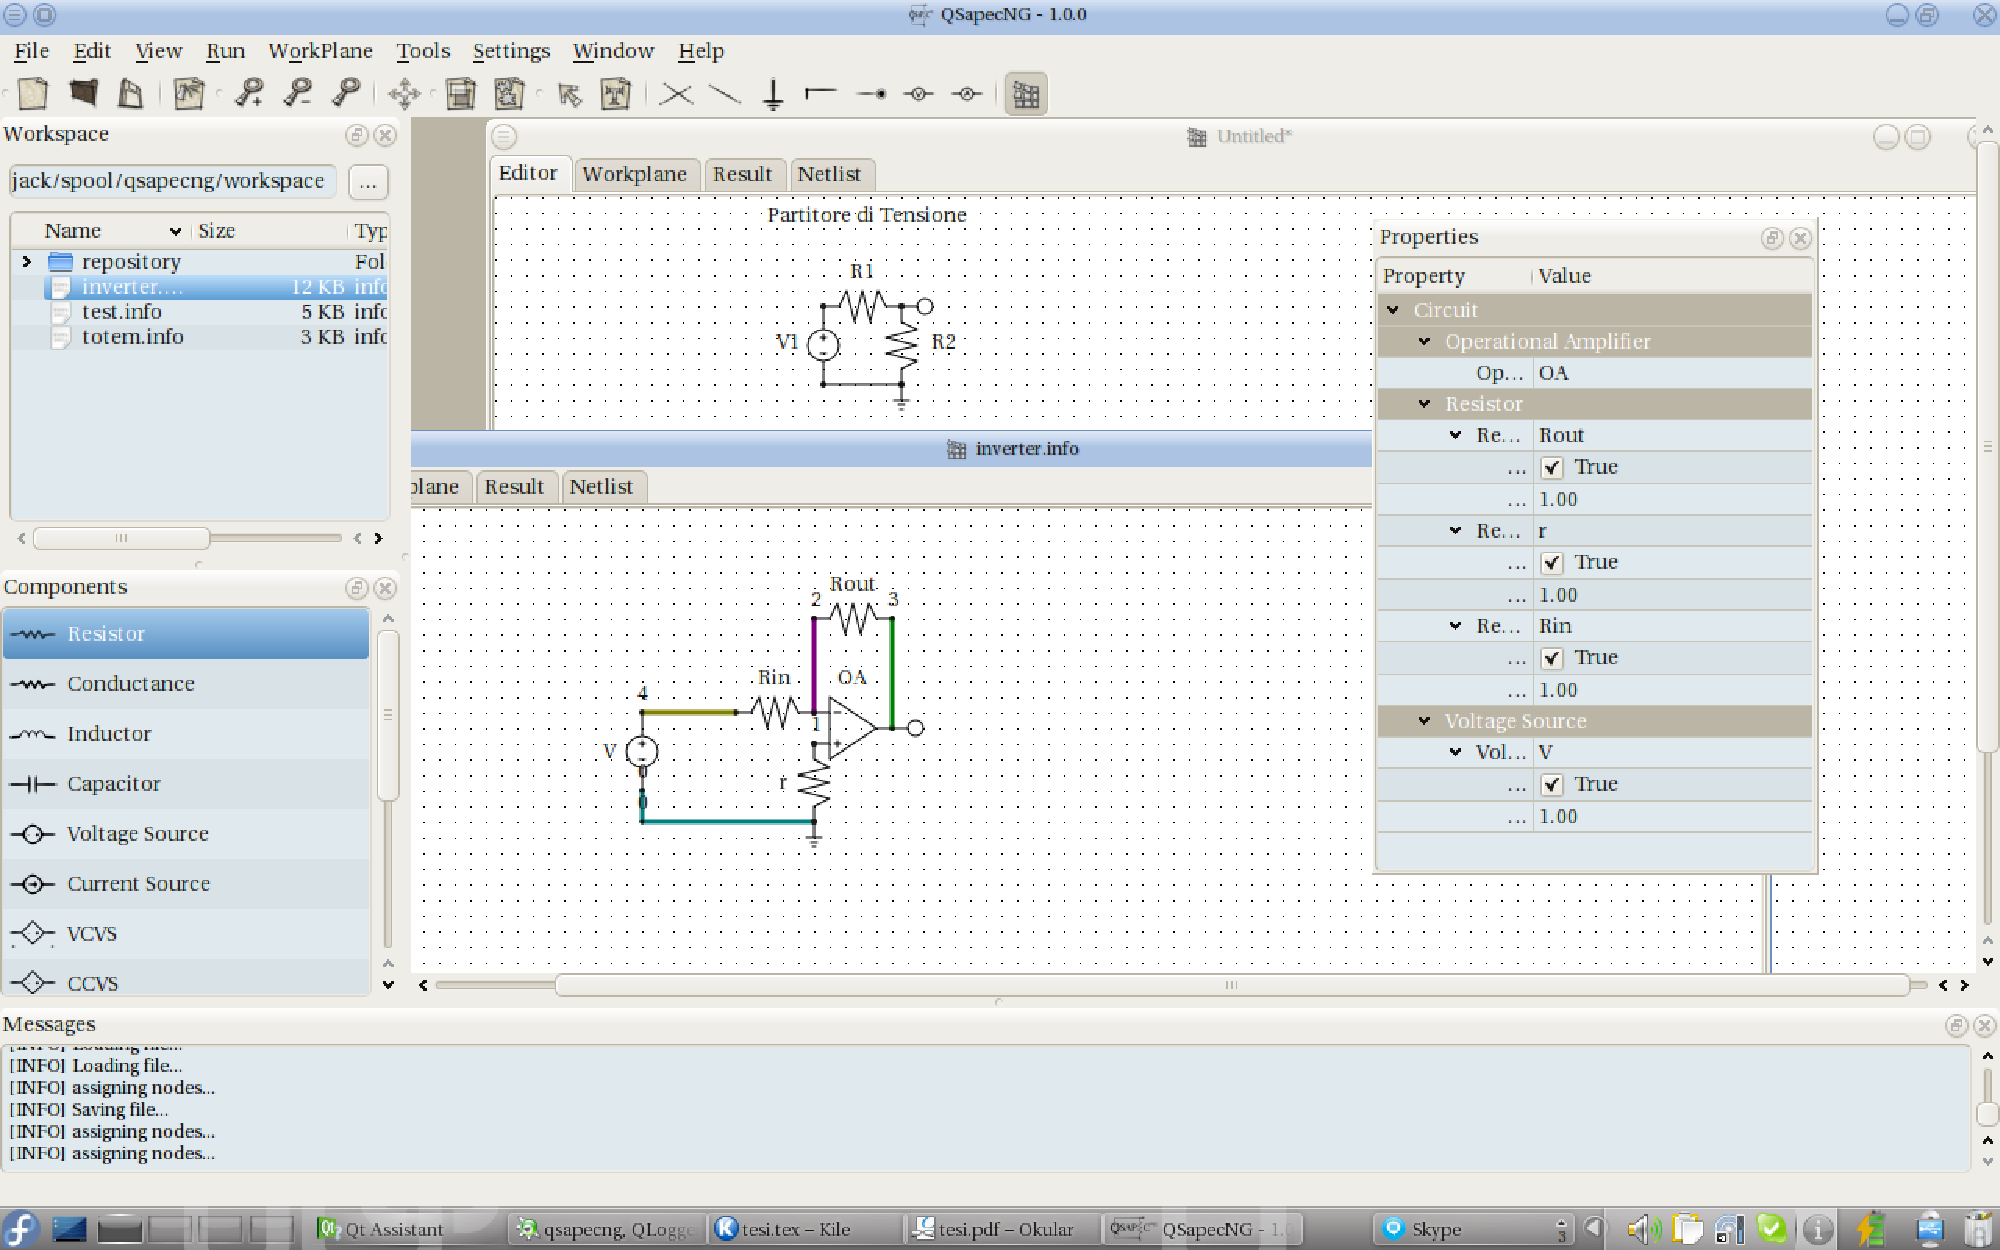
\includegraphics[scale=0.5,angle=90]{immagini/ss1.pdf}}\\
 \caption{QSapecNG (scena)}
 \label{fig:qsapecng-ss}
\end{figure}

In figura \ref{fig:qsapecng-ss} è riportata la scena per il disegno schematico, in due distinti esempi (poiché, ovviamente, è possibile lavorare al contempo su più circuiti diversi). Si può notare come, nelle fasi di risoluzione, i fili vengono colorati e i nodi etichettati con un valore adatto per rendere maggiormente comprensibile la struttura del circuito in esame. Nella stessa immagine si possono inoltre osservare il pannello dei componenti, la barra laterale contenente l'ambiente di lavoro attuale e quella dove vengono riportate per ogni singolo elemento le proprietà associate (quali ad esempio il nome o il valore). Tutti questi pannelli sono mobili e permettono una personalizzazione estrema dell'ambiente di disegno.\\
Un aspetto importante è quello che riguarda l'effettiva risoluzione di un circuito. Essendo QSapecNG sviluppato con tecnologia \textit{multi-threading}, l'analisi di uno schema non bloccherà l'intero software, per quanto questa sia la fase computazionalmente più complessa. Questo si traduce nella possibilità di disegnare circuiti anche molto articolati e, una volta sottomessi al risolutore, dedicarsi al disegno di nuovi schemi senza dover necessariamente aspettare prima che quest'ultimo abbia finito il suo lavoro.

\begin{figure}[hb]
 \centering
 \subfloat{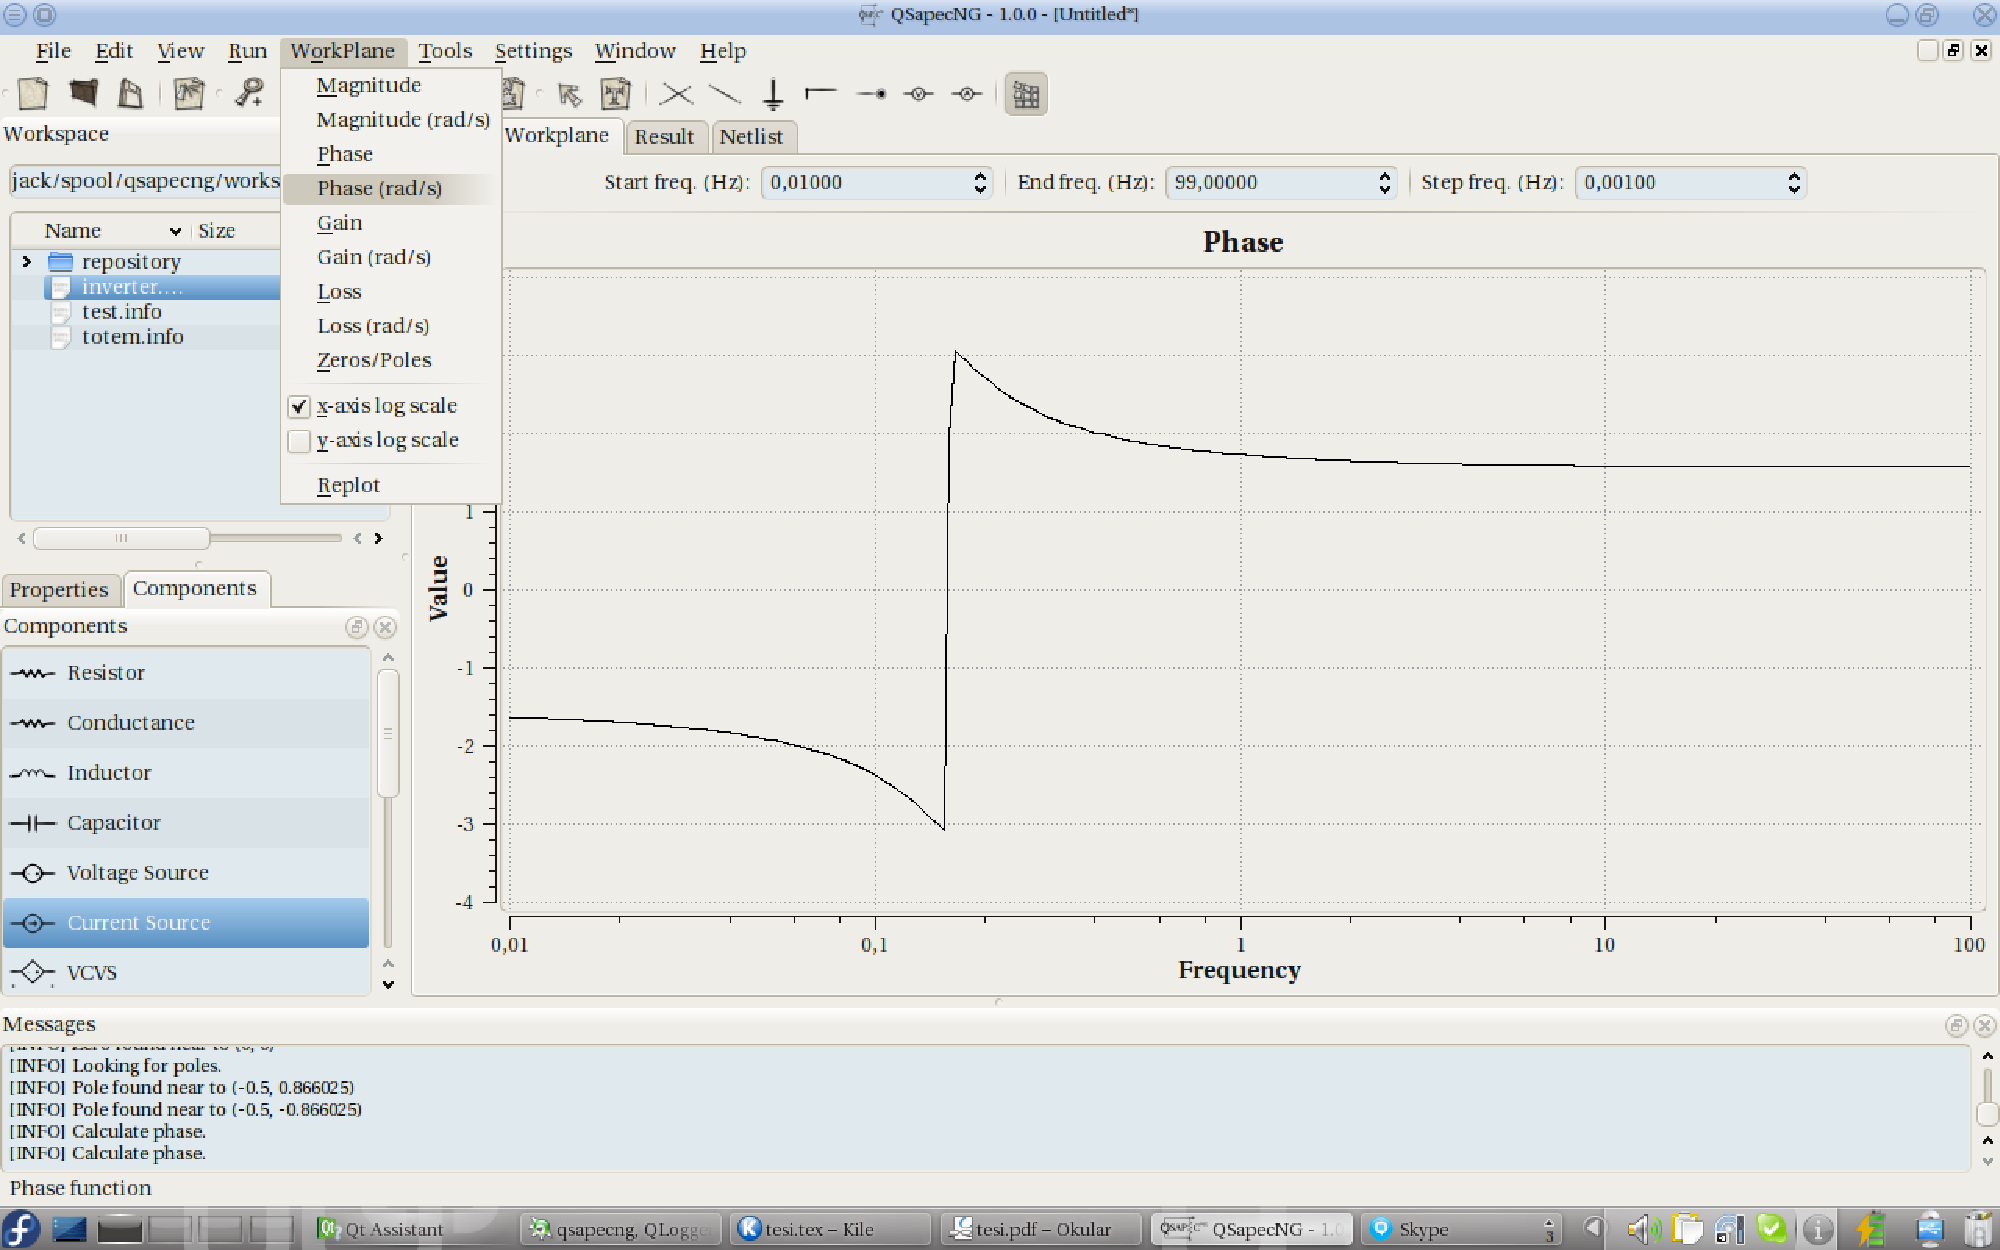
\includegraphics[scale=0.5,angle=90]{immagini/ss2.pdf}}\\
 \caption{QSapecNG (workspace)}
 \label{fig:qsapecng-ws}
\end{figure}

\begin{figure}[ht]
 \centering
 \subfloat{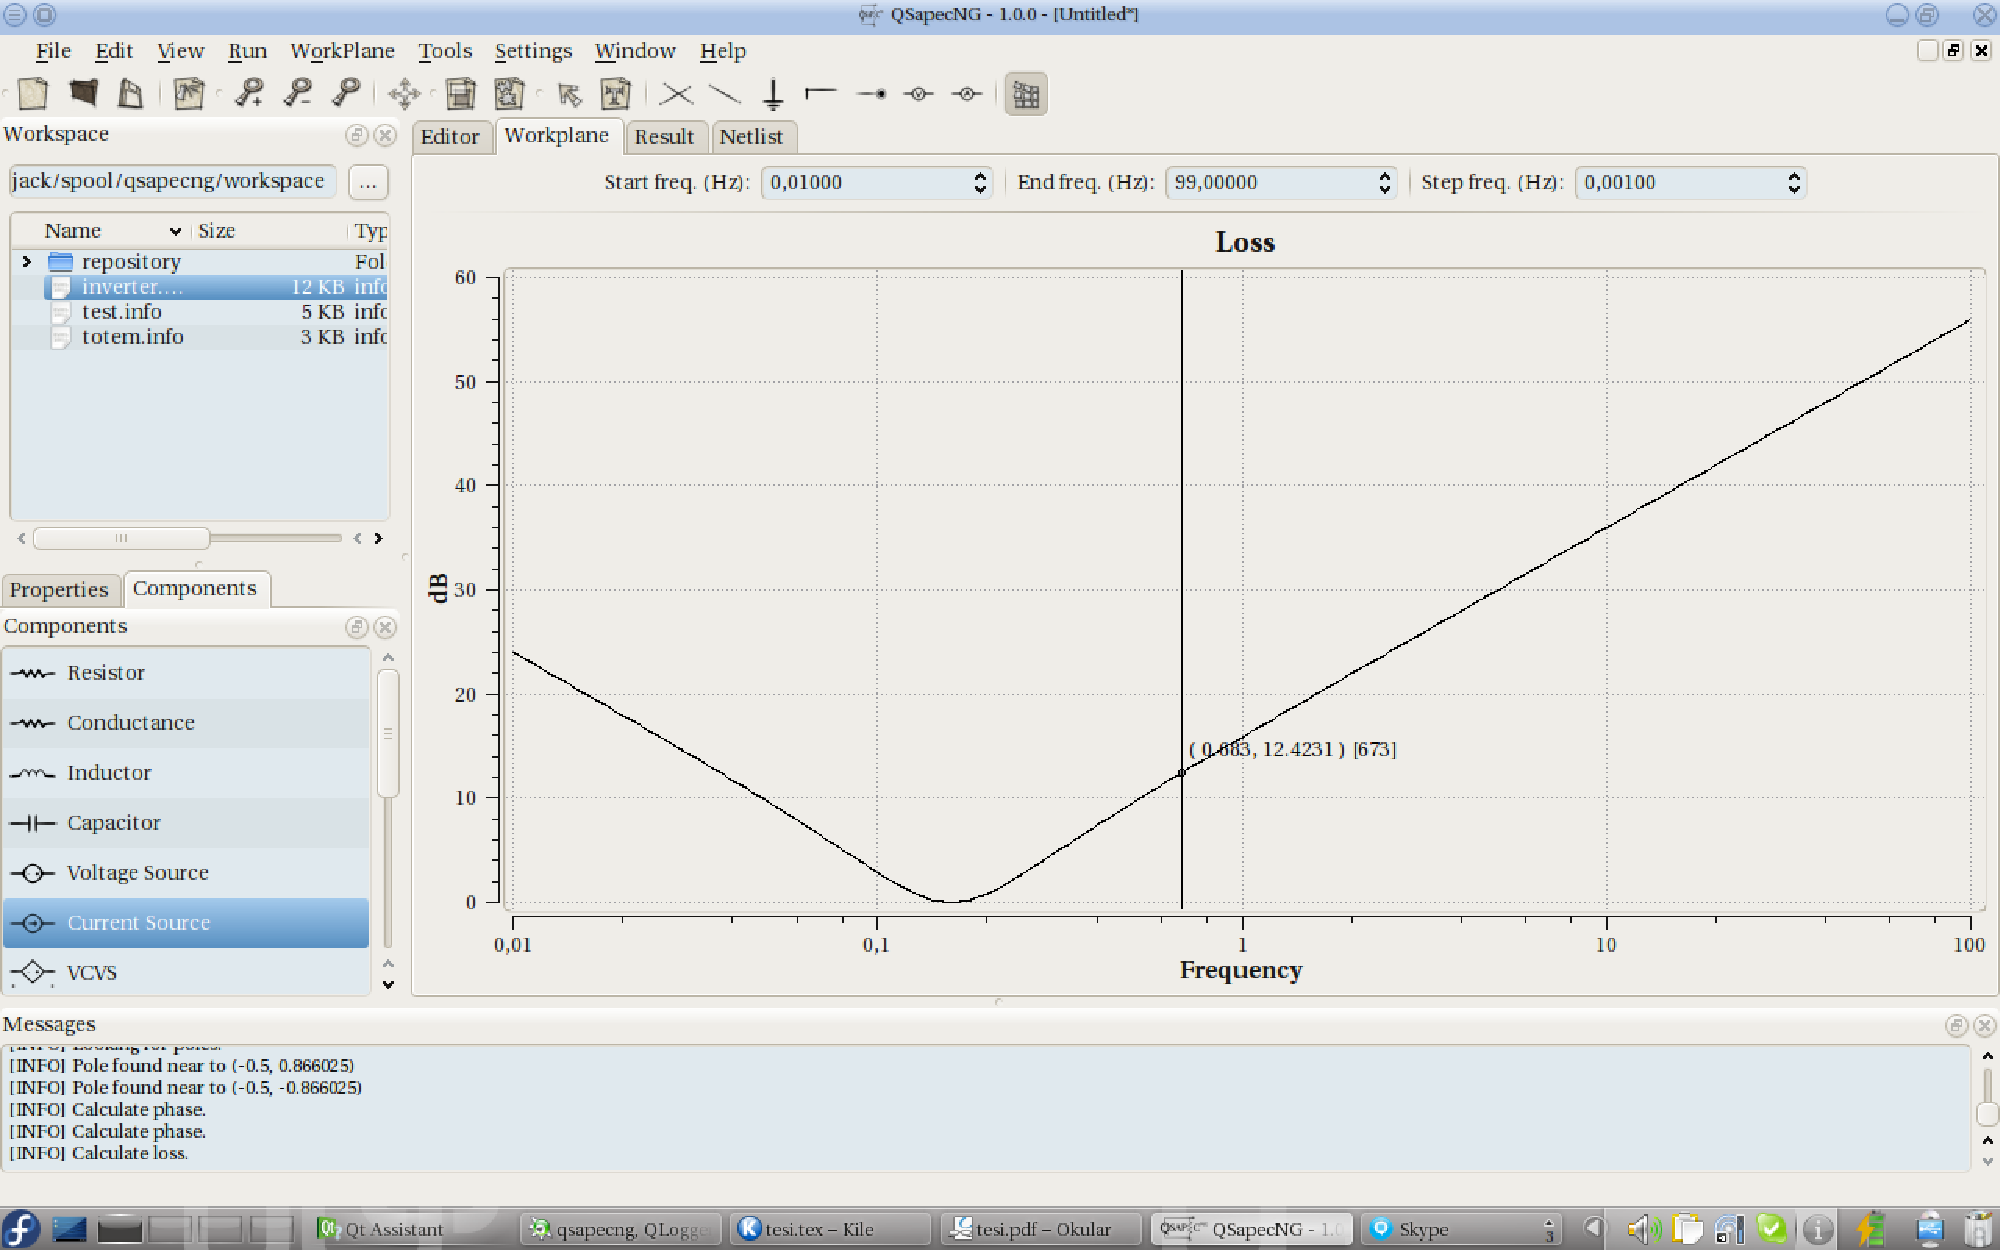
\includegraphics[scale=0.5,angle=90]{immagini/ss3.pdf}}\\
 \caption{QSapecNG (cursore)}
 \label{fig:qsapecng-cur}
\end{figure}

Nelle due figure successive (\ref{fig:qsapecng-ws} e \ref{fig:qsapecng-cur}) è illustrato lo spazio in cui avviene l'analisi della funzione di trasferimento ottenuta. Il numero di funzioni attualmente disponibili è limitato ma in costante crescita e progettato per essere ampliato ad ogni nuova richiesta. Il cursore presente sul grafico permette di avere una visione chiara della curva, disponendo di tutti i valori calcolati (basati sulla frequenza d'inizio, di fine e sul passo) e riportandoli aggiornati ad ogni spostamento.\\
Si noti che per alcune funzioni particolari, come quelle relative al calcolo di poli e zeri, oltre ad avere un rapporto in forma di grafico vi è l'area di \textit{log} del software dove vengono stampati i valori ricavati. Questo, oltre ad agevolare l'accesso ai risultati, permette di leggerli anche qualora finissero col trovarsi al margine dello spazio di disegno, risultando illeggibili. Infatti tali funzioni non mettono a dispozione un cursore ma stampano direttamente sul grafico i pochi valori ottenuti (svincolati in questo caso dalla frequenza di inizio e di fine, oltre che dal passo).

\begin{figure}[ht]
 \centering
 \subfloat{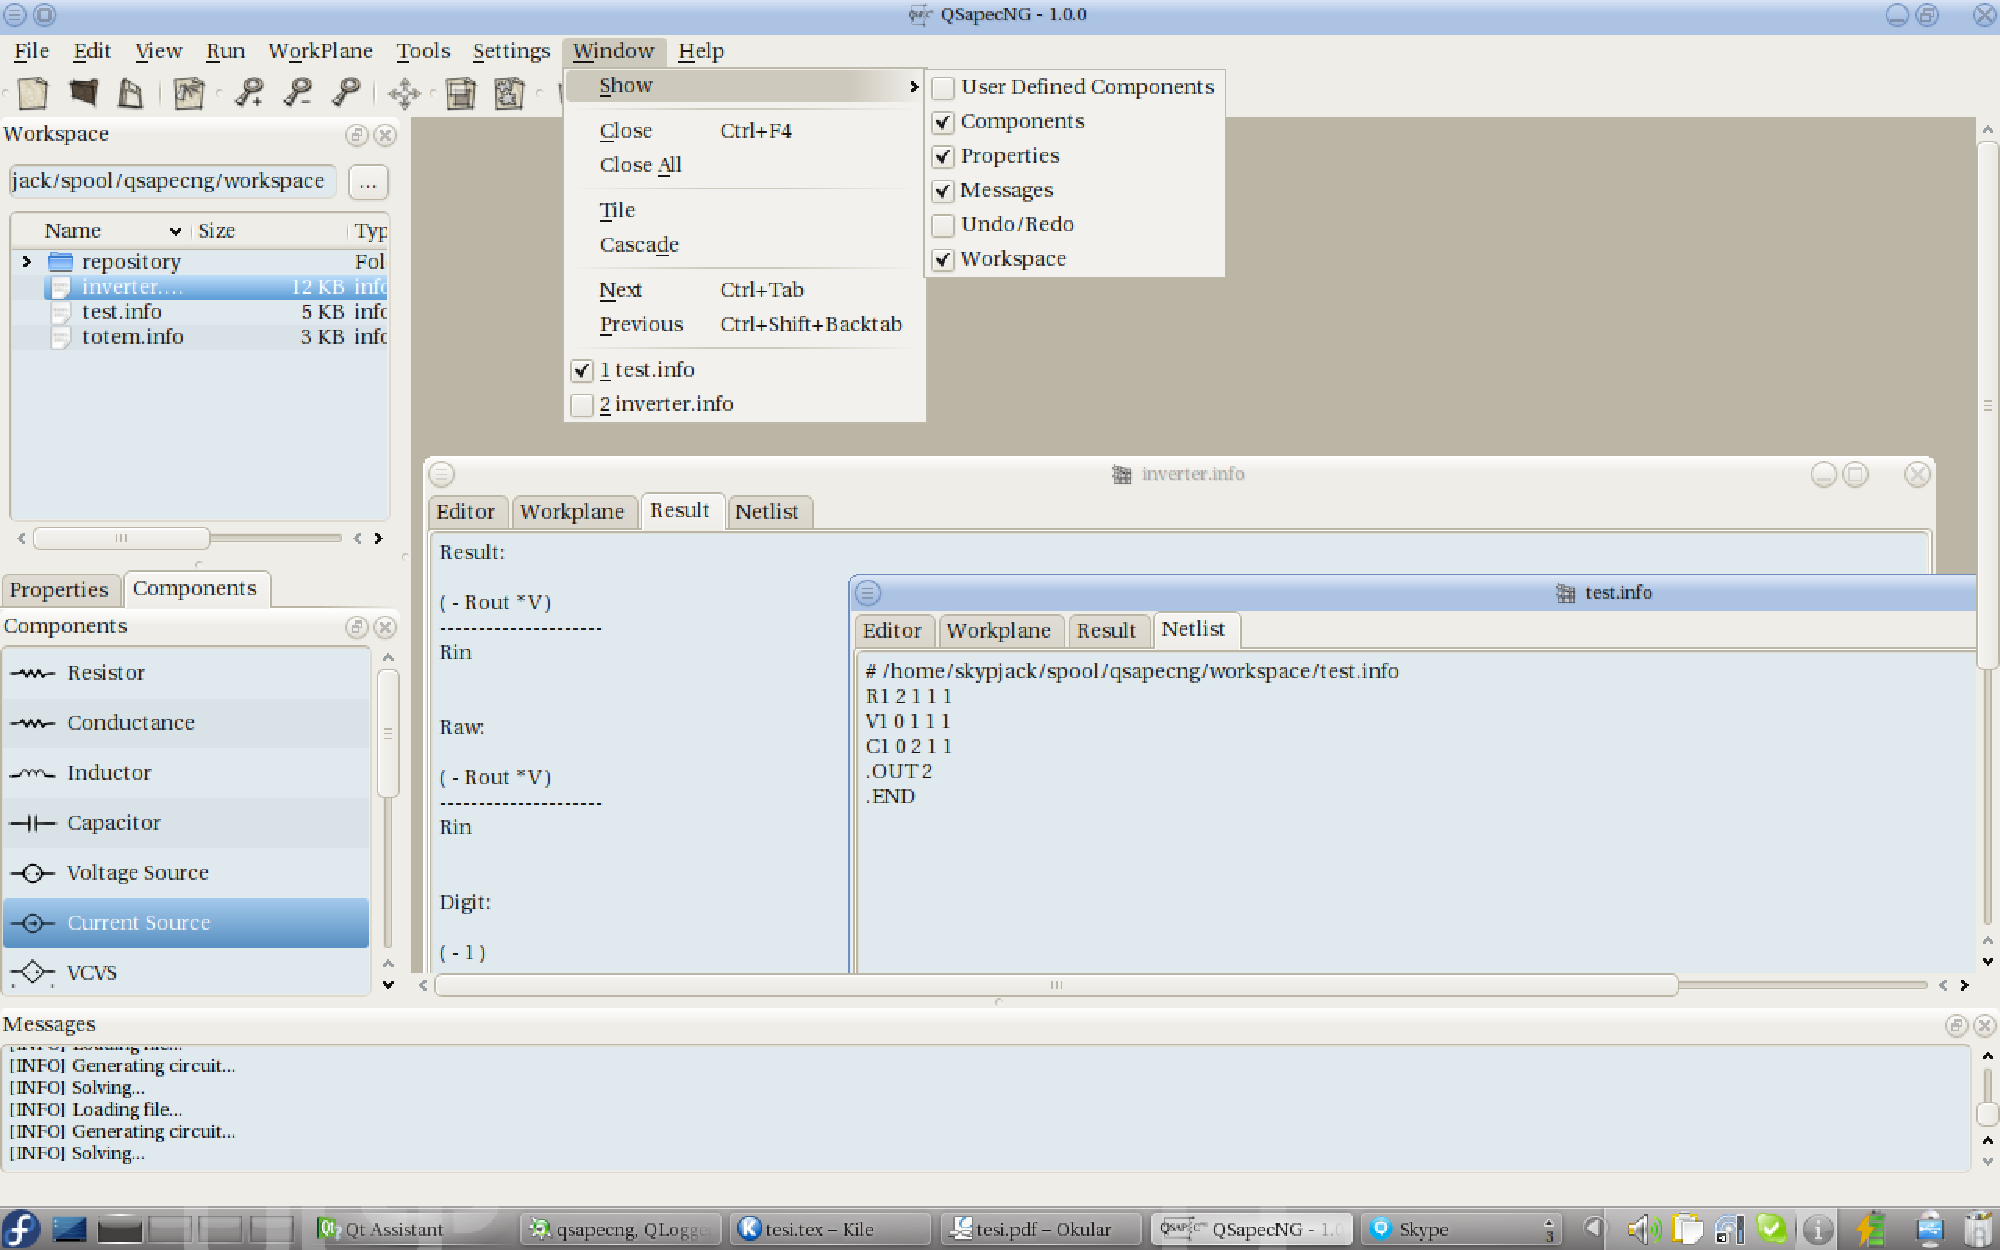
\includegraphics[scale=0.5,angle=90]{immagini/ss4.pdf}}\\
 \caption{QSapecNG (risultati/netlist)}
 \label{fig:qsapecng-resnl}
\end{figure}

In figura \ref{fig:qsapecng-resnl} sono mostrati, in due diverse finestre, alcuni dei risultati ottenibili a partire dallo schema di un circuito.\\
Uno dei più elementari è la traduzione diretta in forma di \textit{netlist}, formato largamente accettato e alla base anche di SapWin. Ogni circuito, all'interno di QSapecNG, all'atto della risoluzione viene tradotto anche in forma di netlist e quindi fornito all'utente per l'uso. Il fatto che ciò avvenga solo ed esclusivamente durante le fasi di risoluzione è strettamente legato alla necessità di avere dei valori ragionevoli per i nodi del circuito, i quali vengono assegnati per propagazione proprio durante le fasi di risoluzione.\\
Altra area importante è la pagina dei risultati dove, una volta risolto il circuito, viene stampata la funzione di trasferimento in forma puramente simbolica, esclusivamente numerica e mista (ques'ultima, sulla base delle richieste dell'utente). Si noti che la prima forma, simbolica, è la stessa che verrà usata all'interno dello spazio di analisi, dove ai marcatori saranno sostituiti i valori effettivi di volta in volta aggiornabili (ovviamente senza richiedere una nuova soluzione del circuito) per poi ricavarne curve di funzioni.

\begin{figure}[ht]
 \centering
 \subfloat{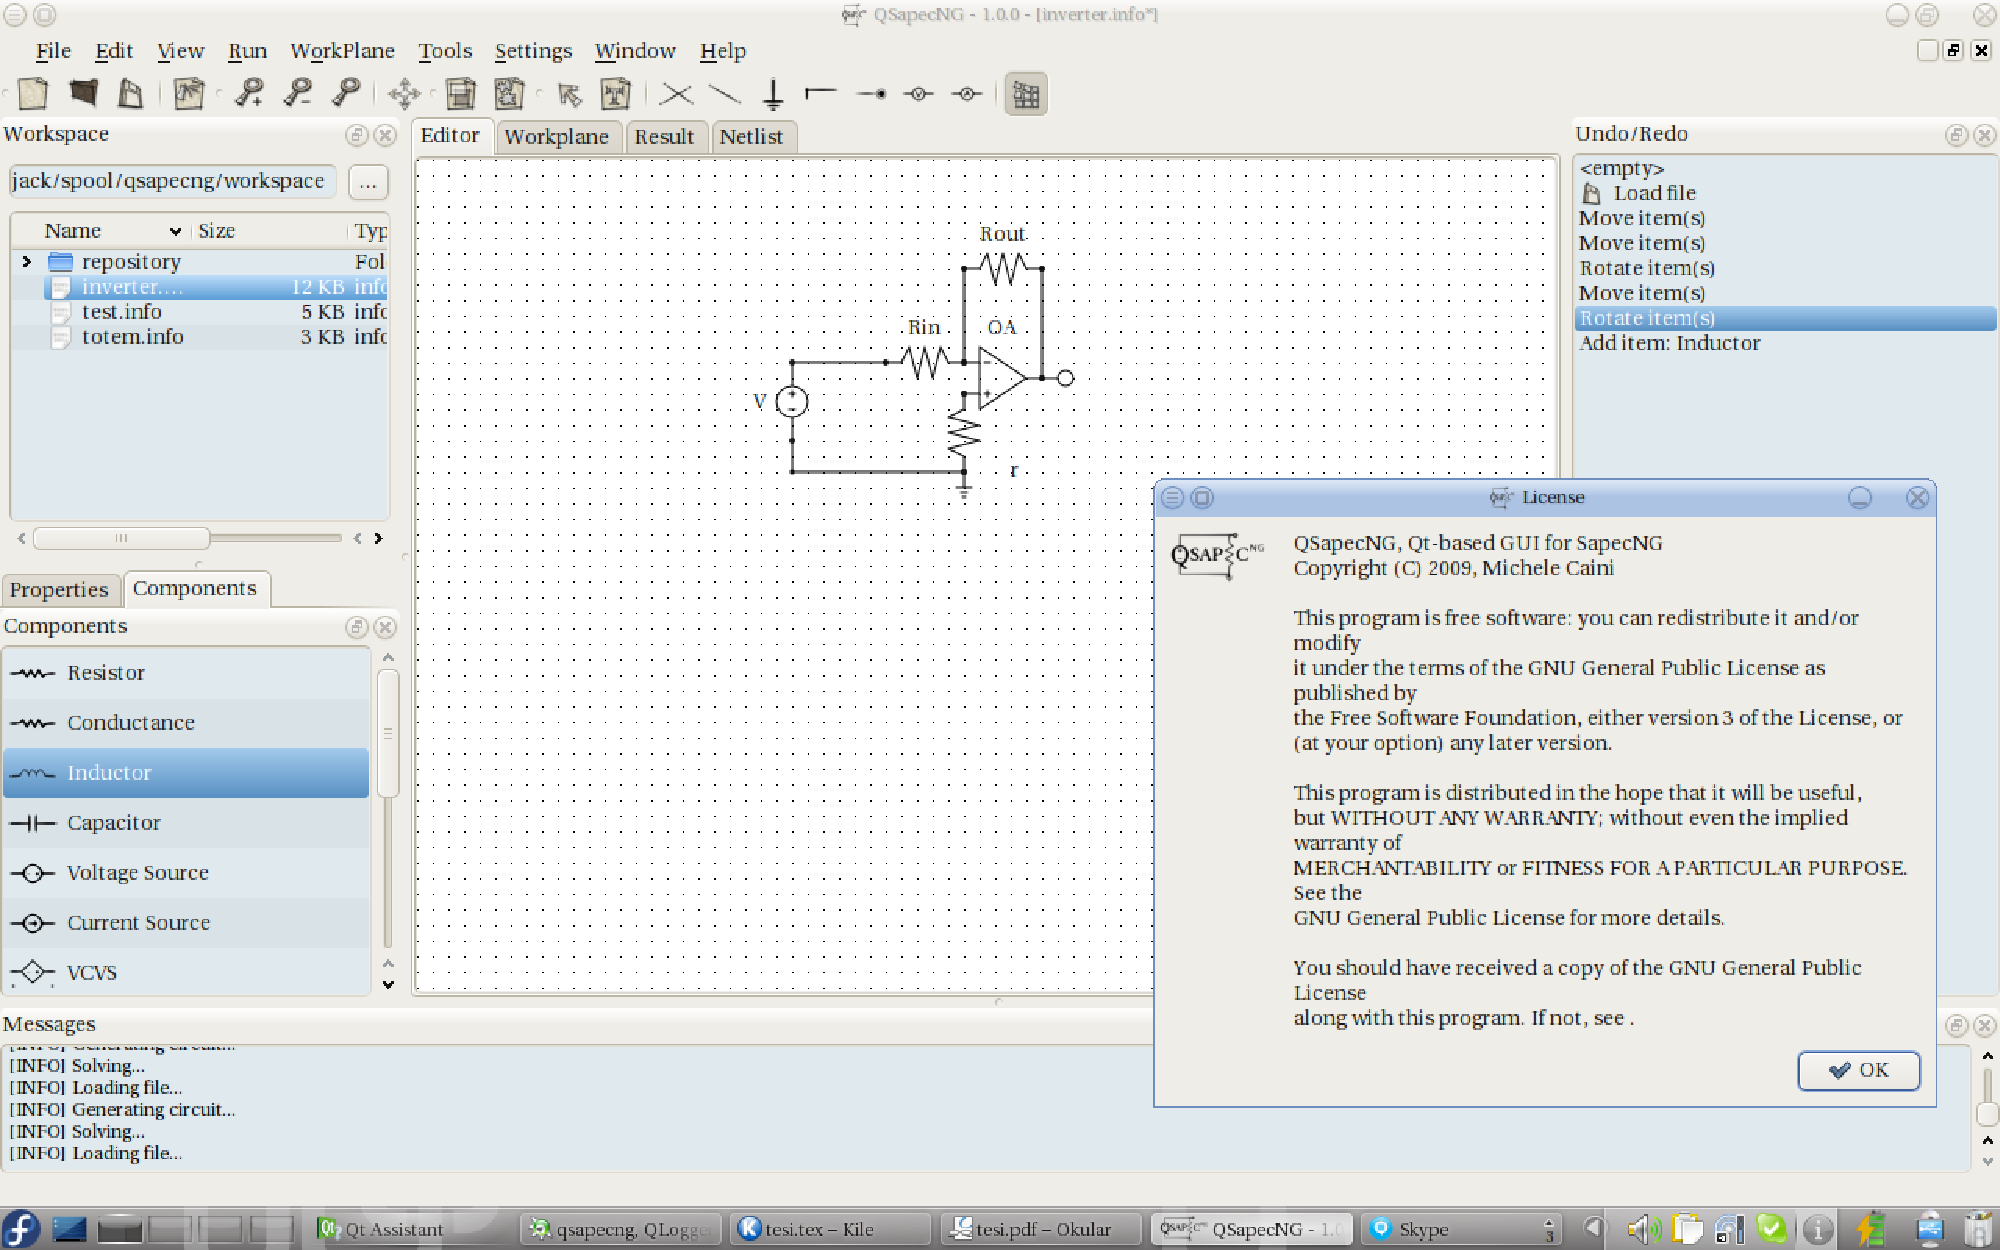
\includegraphics[scale=0.5,angle=90]{immagini/ss5.pdf}}\\
 \caption{QSapecNG (licenza)}
 \label{fig:qsapecng-lic}
\end{figure}

L'ultima immagine, figura \ref{fig:qsapecng-lic}, mostra molto semplicemente la licenza del software e, sullo sfondo, il pannello contenente lo storico delle operazioni per l'\textit{undo-redo}, ovviamente attuabile tramite scorciatoie da tastiera.

\paragraph{}

Quanto sopra è una visione a grandi linee di ciò che offre il software. Ovviamente il tutto non si limita a quanto elencato in questa appendice ma ci sono molti aspetti e dettagli dei quali non vi è modo di discutere in questa sede. Quello che è utile comprendere è che QSapecNG non consiste nel solo risolutore in grado di analizzare un circuito elettrico ma è corredato di un ambiente di sviluppo (per il disegno e l'analisi) completo e progettato con attenzione, ideato con lo scopo di rendere veramente fruibile l'analisi simbolica tanto a coloro che frequentano l'ambiente accademico quanto a coloro che provengono dal mondo aziendale.
